% ------------------------------------------------------------------------------
% TYPO3 CMS 7.2 - What's New (German Version)
%
% @author	Patrick Lobacher <patrick@lobacher.de> and Michael Schams <schams.net>
% @license	Creative Commons BY-NC-SA 3.0
% @link		http://typo3.org/download/release-notes/whats-new/
% @language	German
% ------------------------------------------------------------------------------
% LTXE-CHAPTER-UID:		93899f32-8efb477e-ed6973d2-b679bd8e
% LTXE-CHAPTER-NAME:	Backend User Interface
% ------------------------------------------------------------------------------
% LTXE-SLIDE-START
% LTXE-SLIDE-UID:		c151f95c-3fe3eb42-442ce244-5f987f80
% LTXE-SLIDE-TITLE:		Customized BE login form
% LTXE-SLIDE-REFERENCE:	unknown
% ------------------------------------------------------------------------------
\begin{frame}[fragile]
	\frametitle{Backend User Interface}
	\framesubtitle{Anpassbares Anmeldeformular}

	In der Systemextension \texttt{backend} kann sowohl ein Hintergrundbild,
	ein Logo und die Signalfarbe für die Anmeldeformular eingestellt werden:

	\begin{figure}
		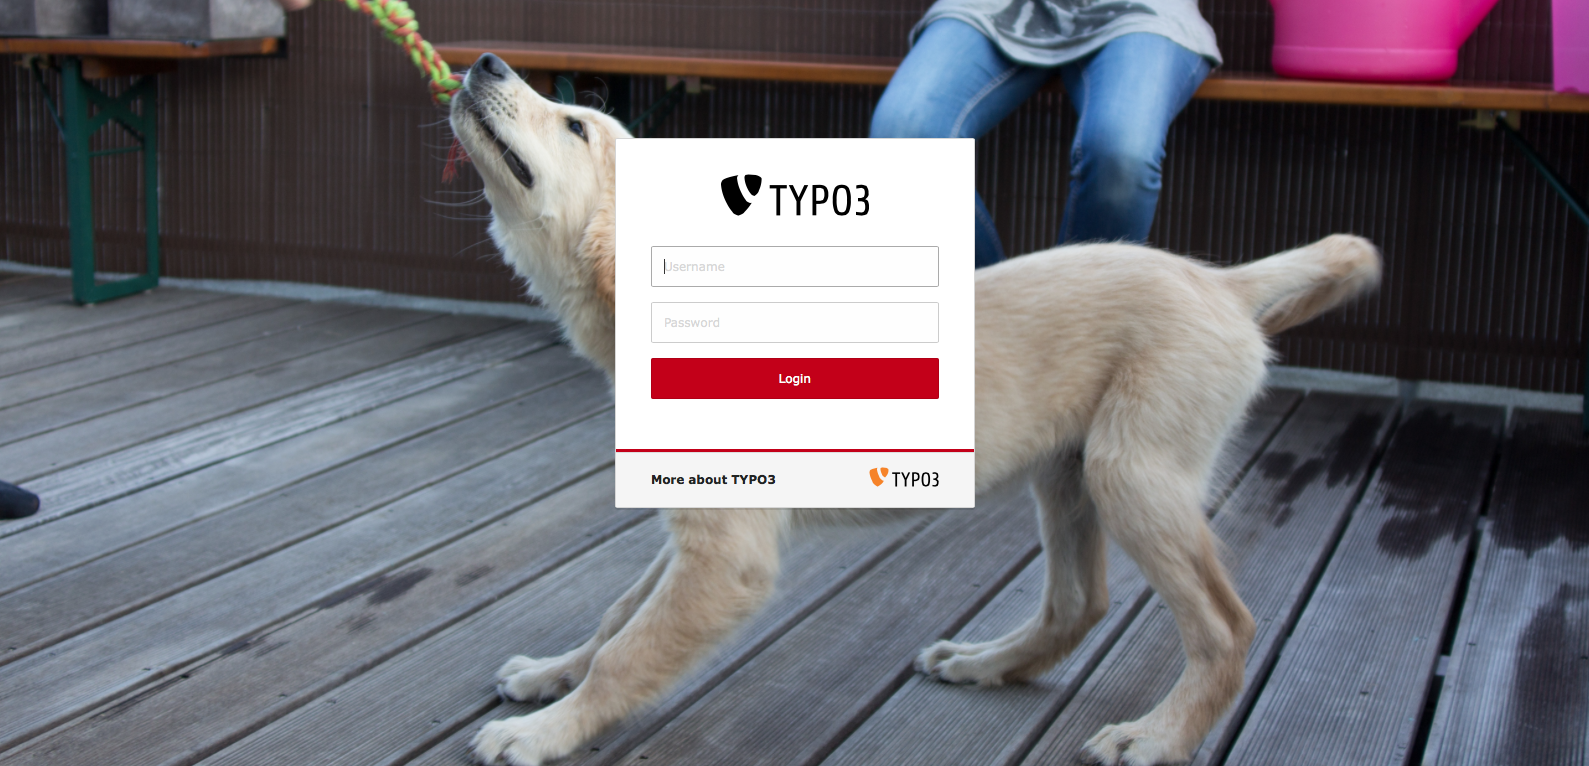
\includegraphics[width=0.75\linewidth]{BackendUserInterface/Login.png}
	\end{figure}

\end{frame}

% ------------------------------------------------------------------------------
% LTXE-SLIDE-START
% LTXE-SLIDE-UID:		e2e353ae-3b2b5c00-0cd7c57d-d97d22c9
% LTXE-SLIDE-TITLE:		Add image cropping
% LTXE-SLIDE-REFERENCE:	Feature-65584-AddImageCropping.rst
% ------------------------------------------------------------------------------
\begin{frame}[fragile]
	\frametitle{Backend User Interface}
	\framesubtitle{Bild-Manipulation (Cropping)}

	Für Bilder kann im Backend bei der Verwendung einer Referenz (z.B. in
	Inhalts-Elementen) ein Ausschnitt ausgewählt werden. Diese Funktion muss
	allerdings für den Redakteur explizit erlaubt werden ("Exclude Fields"):

	\begin{figure}
		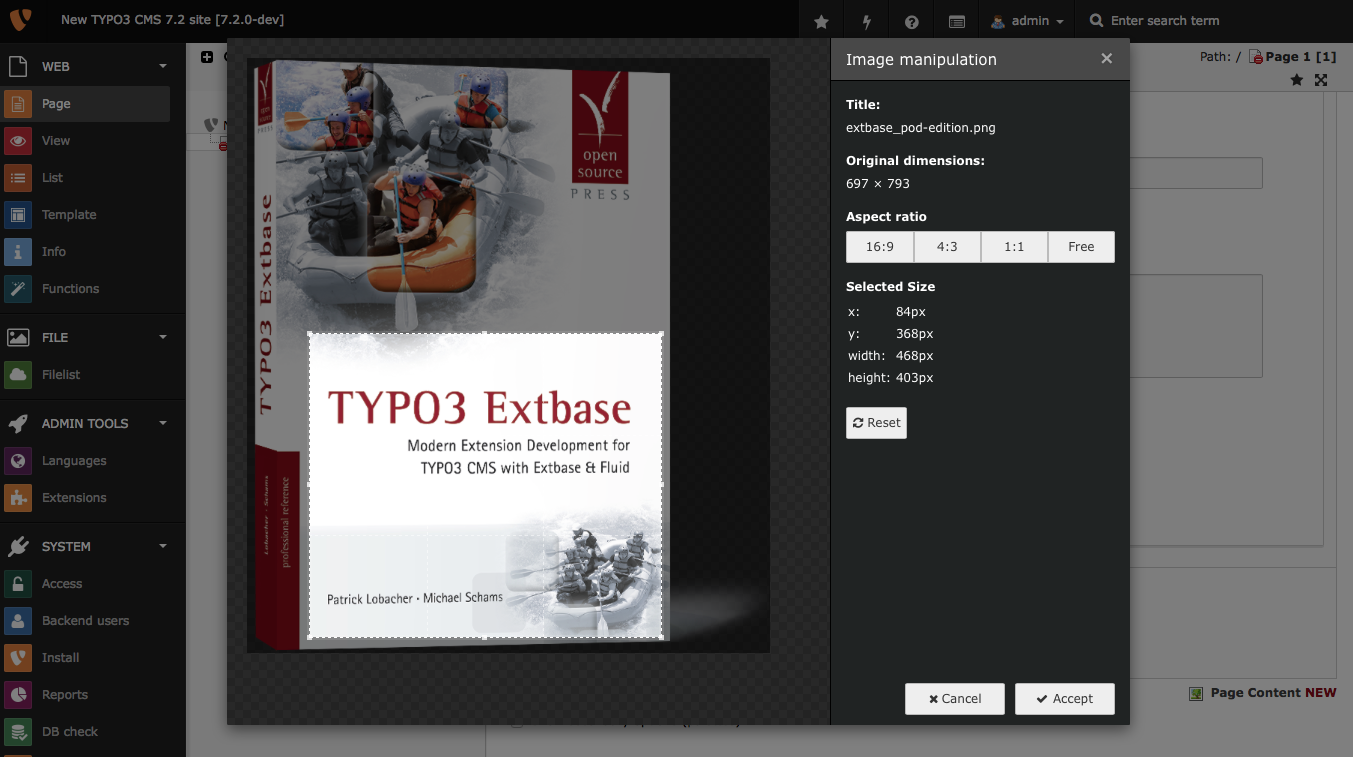
\includegraphics[width=0.7\linewidth]{BackendUserInterface/ImageCropping.png}
	\end{figure}

\end{frame}

% ------------------------------------------------------------------------------
% LTXE-SLIDE-START
% LTXE-SLIDE-UID:		301dfea9-d2debf3e-dcaa7bcd-205e5990
% LTXE-SLIDE-TITLE:		Add backend user groups to backend user module
% LTXE-SLIDE-REFERENCE:	Feature-64686-AddBackendUserGroupsToBackendUserModule.rst
% ------------------------------------------------------------------------------
\begin{frame}[fragile]
	\frametitle{Backend User Interface}
	\framesubtitle{Benutzergruppen}

	Die Backend Benutzergruppen können im Modul "Backend Users" verwaltet werden:

	\begin{figure}
		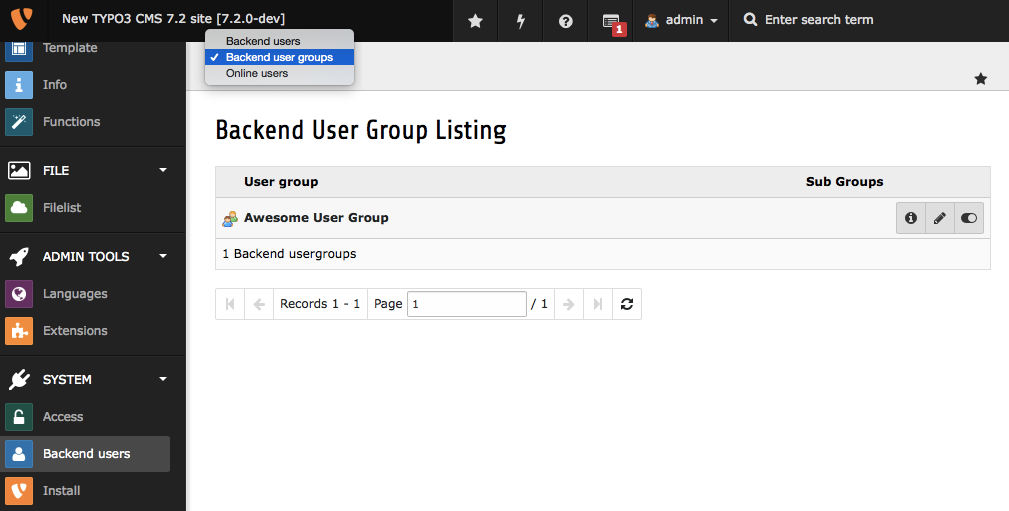
\includegraphics[width=0.70\linewidth]{BackendUserInterface/UserGroups.png}
	\end{figure}

\end{frame}

% ------------------------------------------------------------------------------
% LTXE-SLIDE-START
% LTXE-SLIDE-UID:		daa83c1e-08d2716b-de74cbda-42361551
% LTXE-SLIDE-TITLE:		Extension Manager: Disable automatic installation
% LTXE-SLIDE-REFERENCE:	Feature-50501-DisableAutomaticExtInstallation.rst
% ------------------------------------------------------------------------------
\begin{frame}[fragile]
	\frametitle{Backend User Interface}
	\framesubtitle{Automatische Installationen unterbinden}

	In den Einstellungen des Extension-Managers kann die automatische Installation
	von Extensions nach dem Download deaktiviert werden:

	\begin{figure}
		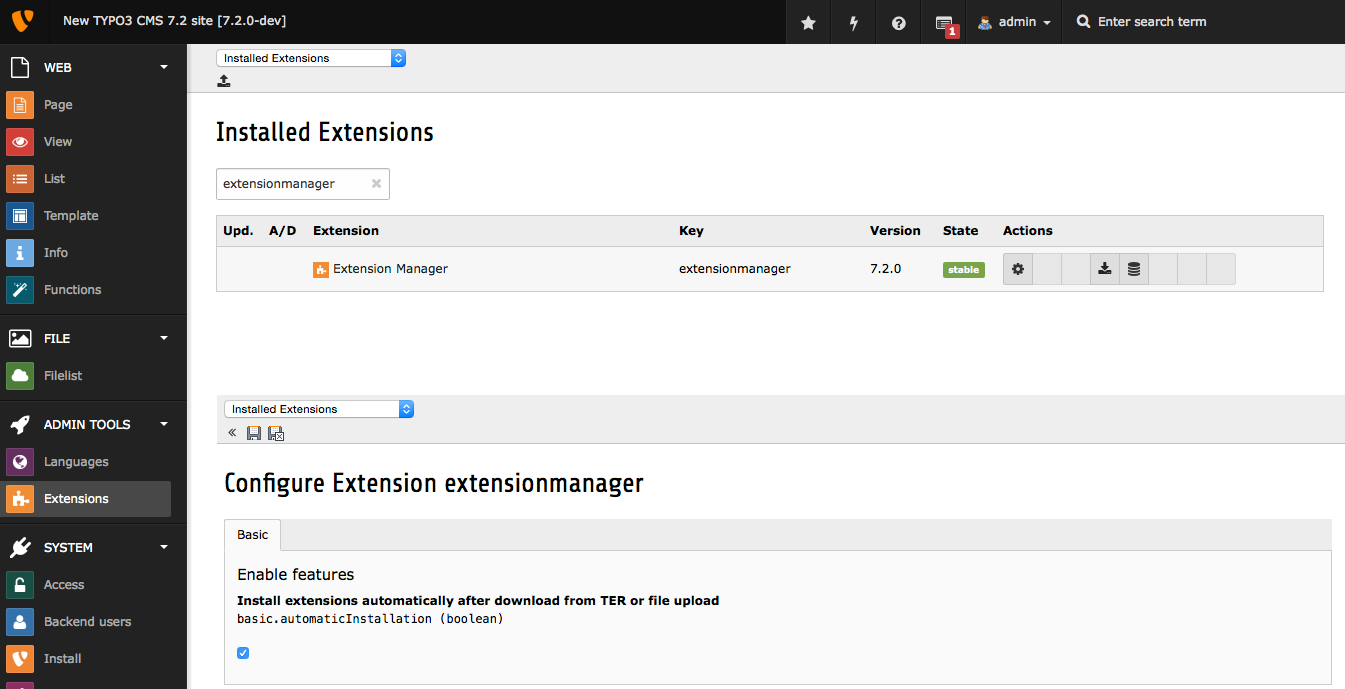
\includegraphics[width=0.70\linewidth]{BackendUserInterface/ExtManager.png}
	\end{figure}

\end{frame}

% ------------------------------------------------------------------------------
% LTXE-SLIDE-START
% LTXE-SLIDE-UID:		20769920-da9df227-c3b527b9-9a23bac1
% LTXE-SLIDE-TITLE:		Show remaining characters below text fields
% LTXE-SLIDE-REFERENCE:	Feature-66029-ShowRemainingCharactersBelowTextFields.rst
% ------------------------------------------------------------------------------
\begin{frame}[fragile]
	\frametitle{Backend User Interface}
	\framesubtitle{Verbleibende Anzahl von Zeichen}

	Unterhalb von Textfeldern wird die verbleibende Anzahl der maximal zulässigen
	Zeichen angezeigt:

	\begin{figure}
		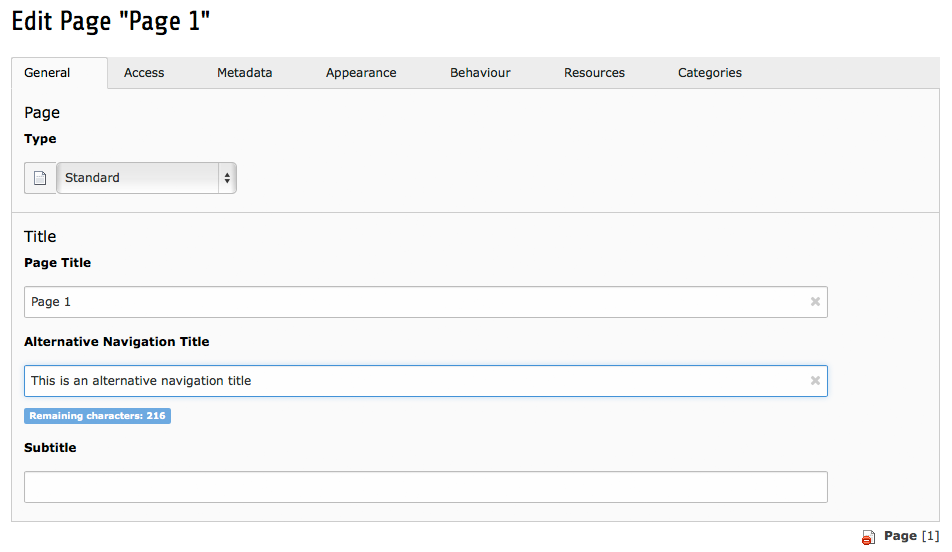
\includegraphics[width=0.70\linewidth]{BackendUserInterface/RemainingCharacters.png}
	\end{figure}

\end{frame}

% ------------------------------------------------------------------------------
% LTXE-SLIDE-START
% LTXE-SLIDE-UID:		ff760b86-9d6b1ecd-d0e98565-f23c51f0
% LTXE-SLIDE-TITLE:		Show confirm message on closing an editform with unsaved changes
% LTXE-SLIDE-REFERENCE:	Feature-65996-AddConfirmationOnCloseEditformWithUnsavedChanges.rst
% ------------------------------------------------------------------------------
\begin{frame}[fragile]
	\frametitle{Backend User Interface}
	\framesubtitle{Ungespeicherte Änderungen}

	Redakteure erhalten eine Warnung, wenn in einem Editier-Formular der "Schließen"-Button
	geklickt wird, ohne vorher gespeichert zu haben:

	\begin{figure}
		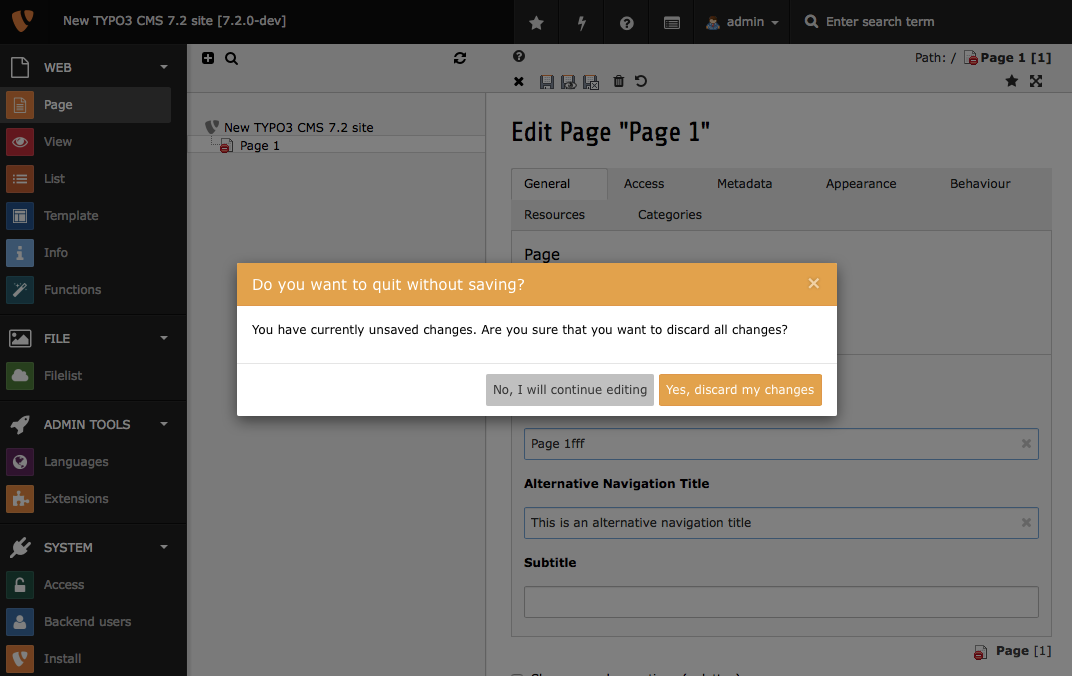
\includegraphics[width=0.65\linewidth]{BackendUserInterface/ClosingDialog.png}
	\end{figure}

\end{frame}

% ------------------------------------------------------------------------------
% LTXE-SLIDE-START
% LTXE-SLIDE-UID:		6ac9a35e-46541895-7509263e-28fb799f
% LTXE-SLIDE-TITLE:		System Information Dropdown
% LTXE-SLIDE-REFERENCE:	Feature-65767-SystemInformationDropdown.rst
% ------------------------------------------------------------------------------
\begin{frame}[fragile]
	\frametitle{Backend User Interface}
	\framesubtitle{Systeminformationen}

	Eine Kurzübersicht der Systeminformationen kann per Klick neben dem Benutzer-Icon
	abgerufen werden. Die Informationen in diesem Dialog sind erweitern (siehe Kapitel
	"Änderungen im System"):

	\begin{figure}
		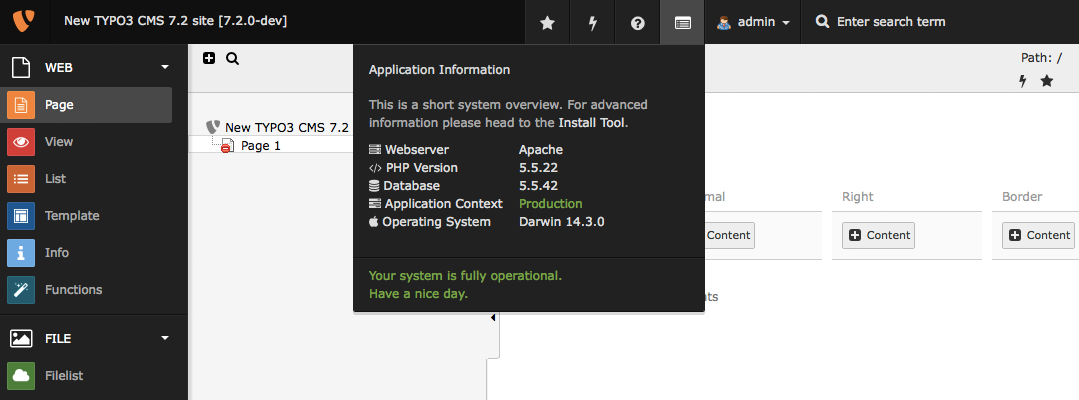
\includegraphics[width=0.85\linewidth]{BackendUserInterface/SystemInformation.png}
	\end{figure}

\end{frame}

% ------------------------------------------------------------------------------
% LTXE-SLIDE-START
% LTXE-SLIDE-UID:		79a2ee0c-3439d600-08990adb-6bed8c19
% LTXE-SLIDE-TITLE:		Ask for old password when changing
% LTXE-SLIDE-REFERENCE:	commit bf6f5226eb6cb441bb53657a88ef42f1cdb5155f
% ------------------------------------------------------------------------------
\begin{frame}[fragile]
	\frametitle{Backend User Interface}
	\framesubtitle{Passwortänderung}

	Zur Änderung des Passwortes müssen Backendbenutzer zuerst ihr aktuelles, altes
	Passwort eingeben:

	\begin{figure}
		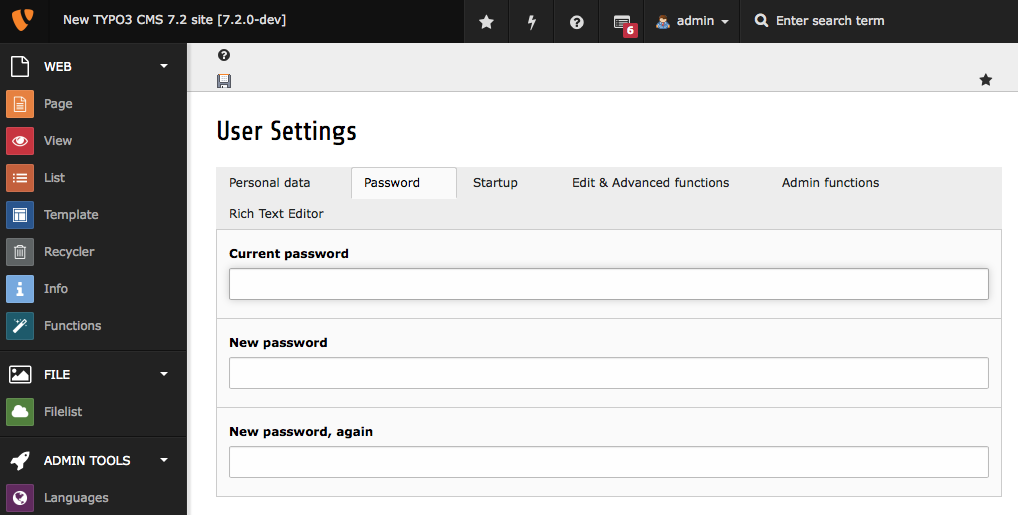
\includegraphics[width=0.7\linewidth]{BackendUserInterface/Password.png}
	\end{figure}

\end{frame}

% ------------------------------------------------------------------------------
% LTXE-SLIDE-START
% LTXE-SLIDE-UID:		7725bce9-e606f055-bf2e7b4a-e870fe2a
% LTXE-SLIDE-TITLE:		Add icon for "Show Content From Page"
% LTXE-SLIDE-REFERENCE:	commit f8aa3eea9aed97a901ef0c3e7c650e1218839596
% ------------------------------------------------------------------------------
\begin{frame}[fragile]
	\frametitle{Backend User Interface}
	\framesubtitle{Icon für "Show Content from Page"}

	Im Seitenbaum zeigt ein neues Icon an, ob eine Seite Inhalte von einer anderen
	Seite enthält ("Show Content from Page"):

	\begin{figure}
		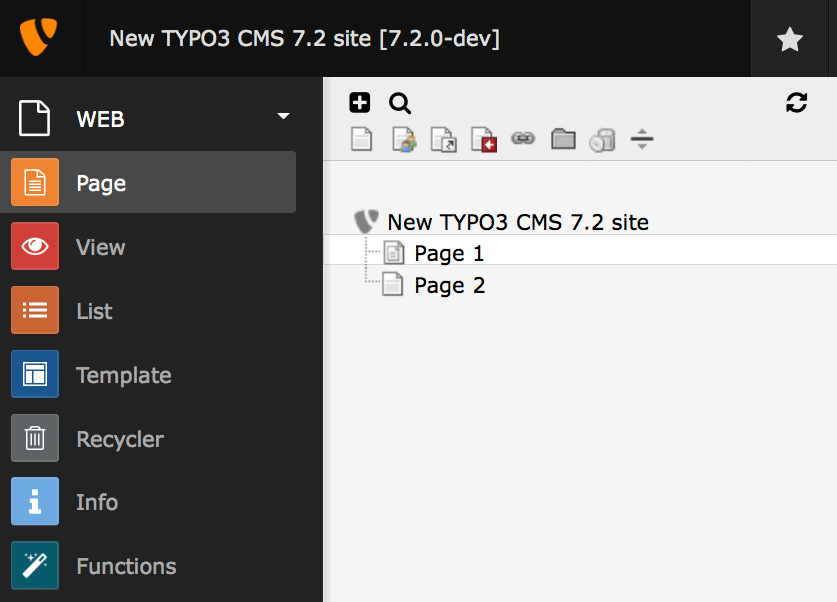
\includegraphics[width=0.45\linewidth]{BackendUserInterface/ShowContent.png}
	\end{figure}

\end{frame}

% ------------------------------------------------------------------------------
% LTXE-SLIDE-START
% LTXE-SLIDE-UID:		5ac2de45-9be12bf9-1c326192-602839fb
% LTXE-SLIDE-TITLE:		EM: Choose version for update
% LTXE-SLIDE-REFERENCE:	commit a26396a4530b530744ec8b36c5fb5606789a6739
% ------------------------------------------------------------------------------
\begin{frame}[fragile]
	\frametitle{Backend User Interface}
	\framesubtitle{Extension Update}

	Beim Update einer Extension wird gefragt, auf welche Version aktualisieren werden soll:

	\begin{figure}
		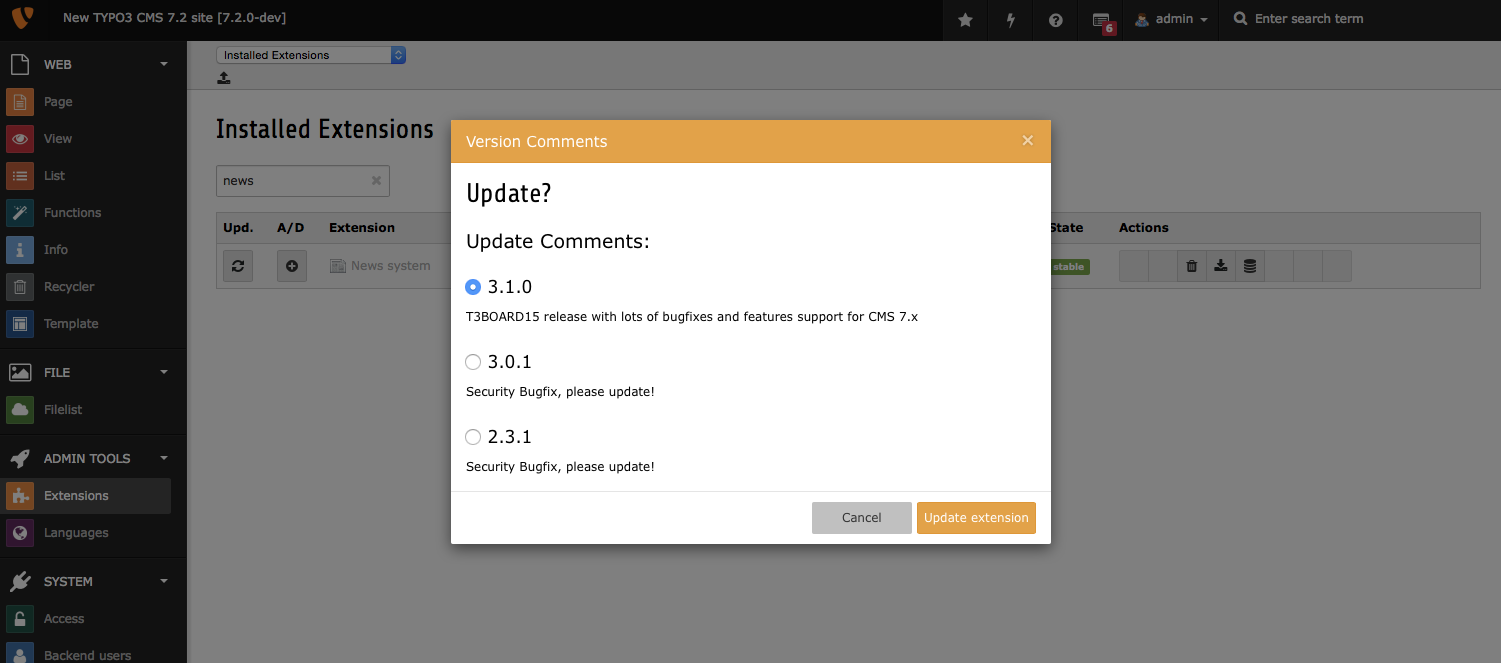
\includegraphics[width=0.75\linewidth]{BackendUserInterface/Update.png}
	\end{figure}

	\small(es wird nicht mehr generell auf die letzte, verfügbare Version aktualisiert)\normalsize

\end{frame}

% ------------------------------------------------------------------------------
% LTXE-SLIDE-START
% LTXE-SLIDE-UID:		f6be31f7-155d676c-0e551545-3fc89e89
% LTXE-SLIDE-TITLE:		Add scheduler task to remove deleted records
% LTXE-SLIDE-REFERENCE:	Feature-32651-AddSchedulerTaskToRemoveDeletedRecords.rst
% ------------------------------------------------------------------------------
\begin{frame}[fragile]
	\frametitle{Backend User Interface}
	\framesubtitle{Recycler Task}

	Die Systemextension \texttt{recycler} bringt nun einen Scheduler Task mit,
	mit dem gelöschte Datensätze aus Content-Tabellen vollständig entfernt werden
	können (inkl. referenzierte Dateien, sofern vorhanden).\newline
	\smaller
		(max. Alter, ab wann Content gelöscht werden kann, ist konfigurierbar)
	\normalsize

	\begin{figure}
		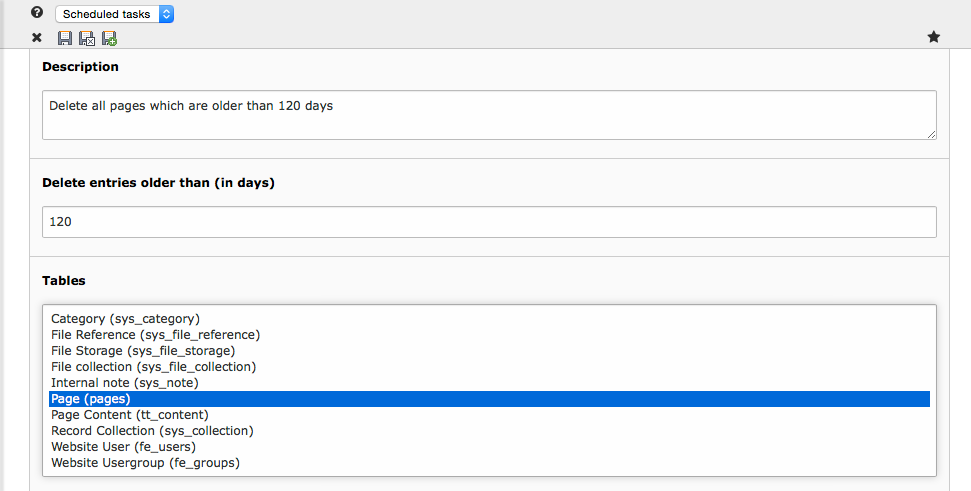
\includegraphics[width=0.68\linewidth]{BackendUserInterface/RecyclerTask.png}
	\end{figure}

\end{frame}

% ------------------------------------------------------------------------------
